%%%%%%%%%%%%%%%%%%%%%%%%%%%%%%%%%%%%%%%%%
% Homework Assignment Article
% LaTeX Template
% Version 1.3.1 (ECL) (08/08/17)
%
% This template has been downloaded from:
% Overleaf
%
% Original author:
% Victor Zimmermann (zimmermann@cl.uni-heidelberg.de)
%
% License:
% CC BY-SA 4.0 (https://creativecommons.org/licenses/by-sa/4.0/)
%
%%%%%%%%%%%%%%%%%%%%%%%%%%%%%%%%%%%%%%%%%

%----------------------------------------------------------------------------------------

\documentclass[a4paper]{article} % Uses article class in A4 format

%----------------------------------------------------------------------------------------
%	FORMATTING
%----------------------------------------------------------------------------------------

\addtolength{\hoffset}{-2.25cm}
\addtolength{\textwidth}{4.5cm}
\addtolength{\voffset}{-3.25cm}
\addtolength{\textheight}{5cm}
\setlength{\parskip}{0pt}
\setlength{\parindent}{0in}

%----------------------------------------------------------------------------------------
%	PACKAGES AND OTHER DOCUMENT CONFIGURATIONS
%----------------------------------------------------------------------------------------

\usepackage{blindtext} % Package to generate dummy text
% \usepackage[style=numeric,sorting=none]{biblatex}
\usepackage{charter} % Use the Charter font
\usepackage[utf8]{inputenc} % Use UTF-8 encoding
\usepackage{microtype} % Slightly tweak font spacing for aesthetics

\usepackage[english]{babel} % Language hyphenation and typographical rules

\usepackage{amsthm, amsmath, amssymb} % Mathematical typesetting
\usepackage{float} % Improved interface for floating objects
\usepackage[final, colorlinks = true, 
            linkcolor = black, 
            citecolor = black]{hyperref} % For hyperlinks in the PDF
\usepackage{graphicx, multicol} % Enhanced support for graphics
\usepackage{xcolor} % Driver-independent color extensions
\usepackage{marvosym, wasysym} % More symbols
\usepackage{rotating} % Rotation tools
\usepackage{censor} % Facilities for controlling restricted text
\usepackage{listings, style/lstlisting} % Environment for non-formatted code, !uses style file!
\usepackage{pseudocode} % Environment for specifying algorithms in a natural way
\usepackage{style/avm} % Environment for f-structures, !uses style file!
\usepackage{booktabs} % Enhances quality of tables
%\usepackage{url}
\usepackage{hyperref}
\usepackage{tikz-qtree} % Easy tree drawing tool
\tikzset{every tree node/.style={align=center,anchor=north},
         level distance=2cm} % Configuration for q-trees
\usepackage{style/btree} % Configuration for b-trees and b+-trees, !uses style file!

% \usepackage[backend=biber,style=numeric,
            % sorting=nyt]{biblatex} % Complete reimplementation of bibliographic facilities
% \addbibresource{ecl.bib}
\usepackage{csquotes} % Context sensitive quotation facilities

\usepackage[yyyymmdd]{datetime} % Uses YEAR-MONTH-DAY format for dates
\renewcommand{\dateseparator}{-} % Sets dateseparator to '-'

\usepackage{fancyhdr} % Headers and footers
\pagestyle{fancy} % All pages have headers and footers
\fancyhead{}\renewcommand{\headrulewidth}{0pt} % Blank out the default header
\fancyfoot[L]{School of Computing, Macquarie University} % Custom footer text
\fancyfoot[C]{} % Custom footer text
\fancyfoot[R]{\thepage} % Custom footer text

\usepackage{comment}
\newcommand{\note}[1]{\marginpar{\scriptsize \textcolor{red}{#1}}} % Enables comments in red on margin

%----------------------------------------------------------------------------------------

\begin{document}
%----------------------------------------------------------------------------------------
%	TITLE SECTION
%----------------------------------------------------------------------------------------
\title{COMP3100 project report} % Article title
\fancyhead[C]{}
\hrule \medskip % Upper rule
\begin{minipage}{1\textwidth} % Center of title section
\centering 
\large % Title text size
Assignment 1 \\
Project report: Stage 1\\ % Assignment title and number
COMP3100 Distributed Systems, S1, 2023\\
\normalsize % Subtitle text size
SID: 46131434, Name: Ravi Inder Singh
%%%%\\ % Assignment subtitle
\end{minipage}
\medskip\hrule % Lower rule
\bigskip
%----------------------------------------------------------------------------------------
%	ARTICLE CONTENTS
%----------------------------------------------------------------------------------------
\tableofcontents

\section{Introduction}
\label{sec:section1}
% \addcontentsline{toc}{section}{Introduction}

This is stage 1 of the project. The project focus on the working of a scheduler in a distributed systems. Distributed systems are network of various computing components working together as if a single system. This environment is helpful in resource allocation while scheduling set of jobs. It ensures the system availability and fault tolerance due to readily availability of other nodes/computers in case of breakdown~\cite{splunk_2021_what}. \\ 
\\
This stage looks into the working of server and client using client side simulator. Server gives the list of jobs and client has to do the task of job scheduler.It is achieved using simple yet effective method by using Largest-Round-Robin (LRR) algorithm. In this algorithm, first server with the highest number of cores is chosen and all the jobs are scheduled on the servers of that type ~\cite{arshad_2023_what}. 
\\

The rest of this report is organised into 5 sections. Section 2 gives high level of understanding on the working of the project and technical aspects of it. Section 3 talks about the computing constraints of the project and design philosophy. Section 4 is all about the implementation, technologies and development libraries used. Finally we have list of references and link to \textbf{GitHub} repository. 

\section{System Overview}
\label{sec:section2}

\subsection{}\begin{figure}
    \centering
    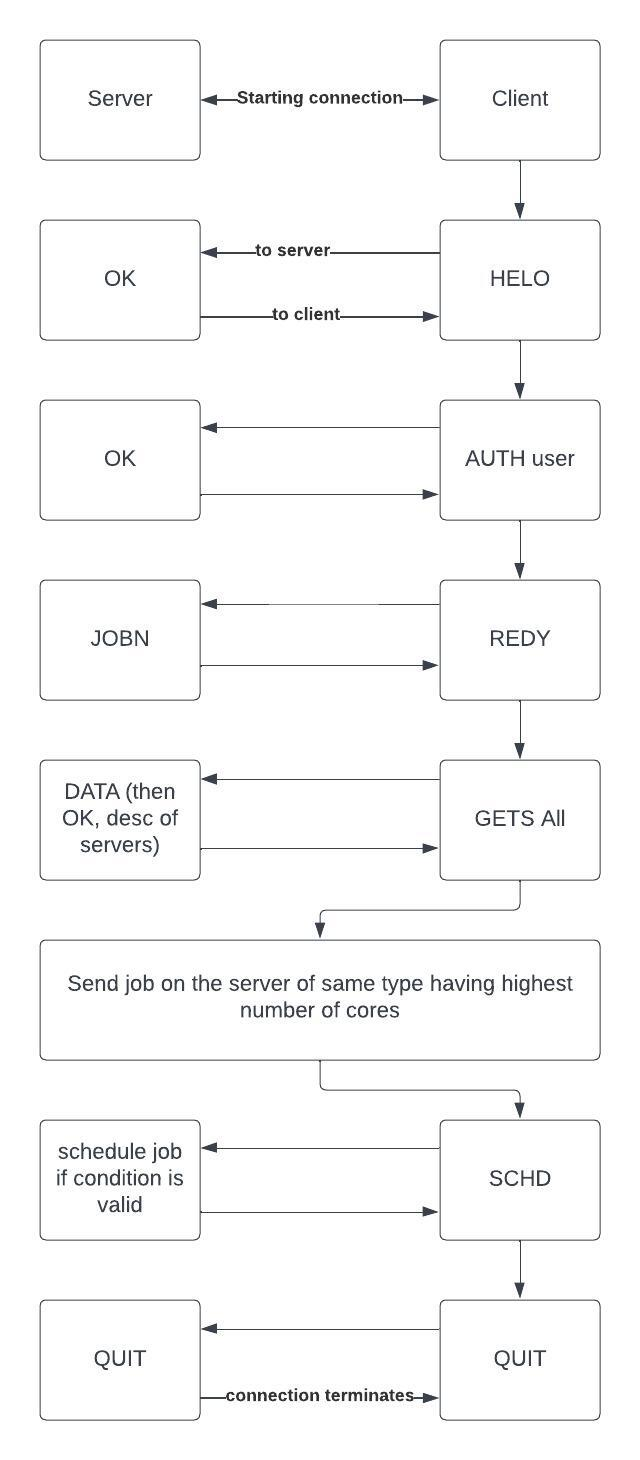
\includegraphics{Pictures/diagram2.jpeg}
    \caption{Workflow}
    \label{fig:my_label}
\end{figure}


\section{Section 3}
\label{sec:section3}
In this section, I first describe x and then y.

\subsection{Section 3.1}
This is a sub-section.

\subsection{Section 3.2}
Yet another sub-section goes here.

\begin{table}[h!]
    \centering
    \begin{tabular}{|c|c|c|c|c|}
    \hline
        Heading 1 & Heading 2 & Heading 3 & Heading 4 & ... \\
    \hline
    A & \$100.0 &&& \\\hline
    B & $\sim$ \$93 &&& \\\hline
    C & $10^2$ &&& \\\hline
    D & $C_2$ &&& \\\hline
    E & 85\% &&& \\\hline
    \end{tabular}
    \label{tab:my_label}
    \caption{Average Performance.}
\end{table}

\subsection{Section 3.3}
Criticism/reflection and improvement suggestions


\section{References}

Link to the \textbf{GitHub} project is \url{https://github.com/Ravi-mq/COMP3100DSAssignment.git}
%----------------------------------------------------------------------------------------
%	REFERENCE LIST
%----------------------------------------------------------------------------------------
\bibliographystyle{ieeetr}
\bibliography{citations}


%----------------------------------------------------------------------------------------

\end{document}
